\section{Buscas}
\begin{frame}

    \frametitle{Buscas}

   \begin{block}{}
     \begin{itemize}
      \item Requisito: conceitos de listas e recursividade  dominados!
      \item  
     \item Essencialmente vamos varrer uma estrutura
     de estados ou nós, de modo sistemático até encontrarmos
     uma solução aceitável.
         

      \item Em geral os problemas 
      se apresentam como uma conexão complexa tipo um \textit{grafo},
      e a varredura sob este grafo é sistemática
      no formato sob uma \textit{árvore de busca}
      
       \item Computar sob listas é o esquema aqui utilizado

    \end{itemize}
    
    \end{block}
    
\end{frame}

\begin{frame}[fragile, allowframebreaks=0.9]
  \frametitle{Ciclo Euleriano}


\begin{figure}[!htb]
\centering
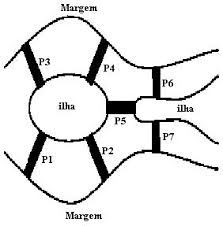
\includegraphics[width=.6\textwidth, height=0.650\textheight]{figures/ilhas_euler.jpeg}
%%%prolog/scale=0.47
%\label{fig_nos_estados}
\caption{Ciclo Euleriano -- Problema das Pontes de Königsberg}
\end{figure}



\framebreak

\begin{itemize}
  \item No século 18 havia na cidade de Königsberg (antiga Prússia)  um conjunto de sete pontes
 (identificadas pelas letras de P1 até P7 na figura ao lado ) que cruzavam o rio  Prególia. 
 Elas conectavam duas ilhas  entre si e as ilhas com as margens esquerda
 e direita.
 
\item Os habitantes daquela cidade perguntavam-se se era possível cruzar 
as sete pontes numa caminhada contínua sem que se passasse duas vezes por 
qualquer uma das pontes.

\item  Embora intrigante, este problema foi atacado por Leonard Euler (1736) e demonstrou
que isto não era possível para um grafo qualquer

\item Curiosamente, este problema, computacionalmente é fácil de resolver!
\end{itemize}

\end{frame}



\begin{frame}[fragile, allowframebreaks=0.9]
  \frametitle{Caminho Hamiltoniano}


\begin{figure}[!htb]
\centering
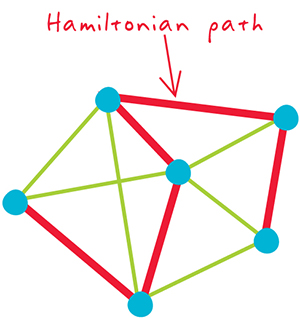
\includegraphics[width=.6\textwidth, height=0.60\textheight]{figures/hamiltonian_path.jpg}
%%%prolog/scale=0.47
%\label{fig_nos_estados}
\caption{Caminho Hamiltoniano -- Há um caminho que passe por todas cidades uma única vez?}
\end{figure}


\framebreak

\begin{itemize}
  \item Diferente do ciclo Euleriano, o caminho Hamiltoniano, origem
  e destino são diferentes
 
\item Todos os nós precisam ser visitados uma única vez sem repetição

\item  Num grafo pode haver muitos caminhos  Hamiltonianos, mas, pode
não existir nenhum!

\item Ao contrário do ciclo Euleriano, este problema, computacionalmente é difícil de resolver!

\item Mas é este que vamos usar como exemplo, com um algoritmo 
bem ingênuo.
\end{itemize}

\end{frame}


\begin{frame}[fragile]
\frametitle{Problemas, Estados, Grafos e  Árvores de Buscas}

\begin{block}{Contextualizando estes termos:}

\begin{itemize}

  \item Em geral, problemas podem ser vistos como \textit{fotografias 
  instantâneas} de uma situação, isto é, \textbf{um estado discreto}
   
  \item Uma sucessão destes estados, compõem \textit{um caminho} de um estado $i$ ao estado $j$
  
  \item Assim, estes estados são representados pelos nós dos grafos, e a ligação entre 
  estes, são resultados de \textit{uma ação}, mudança ou evolução do problema
  
  \item Há um estado particular chamado \textit{inicial}, e algum ou vários outros, os estados \textit{finais}
  
  \item Se o problema tiver várias soluções,  o mesmo apresenta vários caminhos do estado inicial há vários finais.
  
  \item Assim uma sucessão ou transição válida entre estados, é conhecido como uma solução ou instância
     do problema
  
  \item Logo, vamos empregar alguns conceitos de grafos, em modelar problemas e resolvê-los 
  por um esquema de busca computacional
  
\end{itemize}

\end{block}
\end{frame}


%%%%%%%%%%%%%%

\begin{frame}[fragile]
\frametitle{Problemas de Grafos se Transformam em Árvores de Buscas}

\begin{figure}[!htb]
\centering
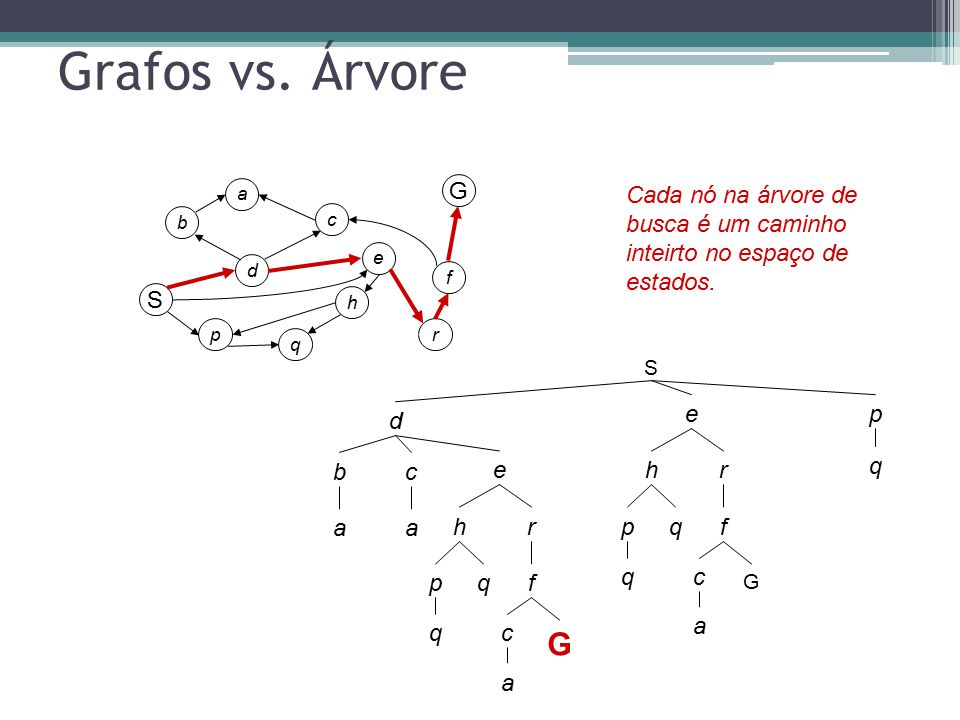
\includegraphics[width=.8\textwidth, height=0.67\textheight]{figures/grafo-arvore-busca.jpg}
%%%prolog/scale=0.47
%\label{fig_nos_estados}
\caption{Refazer esta figura}
\end{figure}

\textcolor{red}{Resumindo, os problemas são modelados  em 
estruturas  complexas, tais como grafos, mas o processo de solução
se mantém: realizar uma busca, tal como uma estrutura de uma árvore }

\end{frame}




\begin{frame}[fragile, allowframebreaks=0.9]
  \frametitle{Núcleo Geral de Buscas}

\textcolor{red}{Pseudo-código já em Picat}

\begin{verbatim}
resolve(P) =>
      inicio(Start),
      busca(Start,[Start],Qsol),
      imprime_saida(Qsol,P).

busca(S,P,P) ?=>  objetivo(S).    % objetivo alcancado : FIM    
busca(S,Visited,P) =>
     proximo_estado(S,Nxt),       % gera um proximo estado  
     estado_seguro(Nxt),          % verifica se este estado é válido 
     sem_loop(Nxt,Visited),       % verifica se está em loop .. repete estados 
     busca(Nxt,[Nxt|Visited],P).  % continue a busca recursiva 
\end{verbatim}


\framebreak


\begin{verbatim}

sem_loop(Nxt,Visited) :-
      \+member(Nxt,Visited).

proximo_estado(S,Nxt) =>   < fill in here >.
estado_seguro(Nxt) =>     < fill in here >.
sem_loop(Nxt,Visited) =>  < fill in here >.     
                       
inicio(...).
objetivo(...).

\end{verbatim}


\textcolor{red}{Vamos reescrever este pseudo-código}


\end{frame}

